\appendix
\section{Theoretical Justification of \cubic}
\label{app:cubic_theory}

This section provides the theoretical justification for the curvature-aware
caching policy used in \cubic. We first analyze the state error induced by
cache reuse and show that it is jointly controlled by local trajectory
curvature and the cache reuse interval. We then convert this error model
into a block-wise interval allocation problem under a global computation
budget and derive the optimal reuse interval. Finally, we show how the
required curvature can be approximated online using endpoint prediction
drift without additional model forward passes.

\subsection{Curvature Approximation}
\label{app:curvature_proxy}

The optimal interval derived in Sec.~\ref{sec:optimizer} depends on the token-wise curvature $\kappa^{(i)}$. Directly computing $\kappa^{(i)}(t)=\|d v_\theta^{(i)}/dt\|_2$, however, requires Jacobian or higher-order derivative information and is therefore expensive for large-scale Flow Matching models. \cubic instead uses endpoint prediction drift as an online curvature proxy.

For a spatial token indexed by $i$, define the one-step endpoint prediction at time $t$ as
\begin{equation}
    \hat{x}_1^{(i)}(t)
    =
    x^{(i)}(t)
    +
    (1-t)
    v_\theta^{(i)}(x(t),t).
    \label{eq:app_endpoint_pred}
\end{equation}
This quantity is the endpoint that would be reached at $t=1$ if the current velocity were kept constant. If the local trajectory is nearly linear, endpoint predictions at nearby times should remain almost unchanged. In contrast, a curved trajectory produces a noticeable endpoint drift.

Taking the total derivative of Eq.~\eqref{eq:app_endpoint_pred} along the exact trajectory gives
\begin{align}
    \frac{d \hat{x}_1^{(i)}}{dt}
    &=
    \frac{d x^{(i)}}{dt}
    -
    v_\theta^{(i)}(x(t),t)
    +
    (1-t)
    \frac{d v_\theta^{(i)}}{dt}
    \nonumber \\
    &=
    (1-t)
    \frac{d v_\theta^{(i)}}{dt}.
    \label{eq:app_endpoint_derivative}
\end{align}
Let $t_{a_{m-1}}$ and $t_{a_m}$ be two consecutive anchor steps, and denote $\Delta t_{a_m}=t_{a_m}-t_{a_{m-1}}$. A first-order Taylor expansion gives
\begin{equation}
    \hat{\delta}^{(i,m)}
    =
    \hat{x}_1^{(i)}(t_{a_m})
    -
    \hat{x}_1^{(i)}(t_{a_{m-1}})
    \approx
    (1-t_{a_m})
    \frac{d v_\theta^{(i)}}{dt}(t_{a_m})
    \Delta t_{a_m}.
\end{equation}
Taking norms yields
\begin{equation}
    \left\|
    \hat{\delta}^{(i,m)}
    \right\|_2
    \approx
    (1-t_{a_m})
    \Delta t_{a_m}
    \kappa^{(i)}(t_{a_m}).
    \label{eq:app_drift_curvature_relation}
\end{equation}
Therefore, the normalized endpoint drift
\begin{equation}
    \hat{\kappa}^{(i)}
    =
    \frac{
    \left\|
    \hat{\delta}^{(i,m)}
    \right\|_2
    }{
    (1-t_{a_m})\Delta t_{a_m}
    }
    \label{eq:app_kappa_estimator}
\end{equation}
serves as an online approximation of $\kappa^{(i)}(t_{a_m})$.

This proxy uses only quantities already available at anchor steps, namely the current latent state and the model-predicted velocity. It therefore requires no additional model forward passes. 





\subsection{Error Modeling of Cache Reuse}
\label{app:error_modeling}

We first derive the local state error induced by cache reuse at the
position level. Consider a block $b$ that is fully recomputed at time
$t_0$, producing the cached velocity
\begin{equation}
    v_0^{(b)} = v_\theta^{(b)}(x(t_0),t_0).
\end{equation}
If this velocity is reused for the next $\tau_b$ solver steps, the local
approximate dynamics follow a zero-order hold:
\begin{equation}
    \frac{dx_{\textrm{exact}}^{(b)}(t)}{dt}=v_0^{(b)}.
\end{equation}
Let $x_{\textrm{exact}}^{(b)}(t)$ denote the exact trajectory. The cache-induced state
error is
\begin{equation}
    \varepsilon_b(t)
    =
   x_{\textrm{cache}}^{(b)}(t)-x_{\textrm{exact}}^{(b)}(t)
    =
    \int_{t_0}^{t}
    \left[
    v_0^{(b)}-v_\theta^{(b)}(x(t'),t')
    \right]dt'.
\end{equation}

We quantify the local trajectory curvature at block $b$ by the rate of
change of the velocity field along the exact trajectory:
\begin{equation}
    \kappa_b(t)
    =
    \left\|
    \frac{d v_\theta^{(b)}}{dt}(x(t),t)
    \right\|_2 .
    \label{eq:app_curvature_def}
\end{equation}
Assume that $\kappa_b(t)\le \bar{\kappa}_b$ within the reuse window. Then
the velocity mismatch satisfies
\begin{equation}
    \left\|
    v_0^{(b)}-v_\theta^{(b)}(x(t),t)
    \right\|_2
    \le
    \bar{\kappa}_b(t-t_0).
\end{equation}
Integrating over a reuse window of length $\tau_b\Delta t$ gives
\begin{equation}
    \left\|\varepsilon_b(t_0+\tau_b\Delta t)\right\|_2
    \le
    \frac{1}{2}
    \bar{\kappa}_b
    \tau_b^2
    \Delta t^2 .
    \label{eq:app_zoh_error_bound}
\end{equation}


The measured cache-induced error follows an approximate power-law dependence on both the reuse interval $\tau$ and the local curvature proxy $\kappa$, supporting the error bound in Eq.~\eqref{eq:app_zoh_error_bound}.

Therefore, cache reuse introduces a state error that grows linearly with
local curvature and quadratically with the reuse interval. Taking the
squared norm as the cache-loss surrogate gives
\begin{equation}
    \ell_b(\tau_b)
    =
     \left\|\varepsilon_b(t_0+\tau_b\Delta t)\right\|_2^2
    \lesssim
    \frac{1}{4}
    \bar{\kappa}_b^2
    \tau_b^4
    \Delta t^4 .
\end{equation}
Dropping shared constants yields the default surrogate
\begin{equation}
    \ell_b(\tau_b)
    \propto
    \kappa_b^2 \tau_b^4 .
    \label{eq:app_surrogate_default}
\end{equation}
More generally, we write
\begin{equation}
    \ell_b(\tau_b)
    =
    a_b
    \kappa_b^\alpha
    \tau_b^\beta ,
    \label{eq:app_general_surrogate}
\end{equation}
where the theoretical default is $(\alpha,\beta)=(2,4)$.
\subsection{Optimal Cache Reuse Interval under a Target Speedup}
\label{app:optimal_interval}

We next derive the optimal block-wise reuse interval under a target
speedup. Let $\tau_b$ denote the update interval of block $b$, and let
$\mathcal{B}_b$ be the set of  tokens contained in this block.
Since different blocks may contain different numbers of tokens, both the
cache-induced error and the computation reduction should be weighted by
the block size $|\mathcal{B}_b|$.

Using the generalized cache-loss surrogate from
Eq.~\eqref{eq:app_general_surrogate}, we consider the following
block-weighted optimization problem:
\begin{equation}
    \min_{\{\tau_b\}_{b=1}^{B}}
    \sum_{b=1}^{B}
    |\mathcal{B}_b|
    \kappa_b^\alpha
    \tau_b^\beta,
    \qquad
    \mathrm{s.t.}
    \quad
    \sum_{b=1}^{B}
    \frac{|\mathcal{B}_b|}{N}
    \frac{1}{\tau_b}
    =
    \frac{1}{\rho},
    \quad
    \tau_b\ge 1,
    \label{eq:app_interval_opt}
\end{equation}
where $N=\sum_{b=1}^{B}|\mathcal{B}_b|$ is the total number of spatial
tokens, $\rho$ is the target speedup, and $\kappa_b$ is the block-wise
curvature estimate. The constraint states that the block-size-weighted
average update rate equals the reciprocal of the target speedup.

Ignoring integer and box constraints, the Lagrangian is
\begin{equation}
    \mathcal{L}
    =
    \sum_{b=1}^{B}
    |\mathcal{B}_b|
    \kappa_b^\alpha
    \tau_b^\beta
    +
    \lambda
    \left(
    \sum_{b=1}^{B}
    \frac{|\mathcal{B}_b|}{N}
    \frac{1}{\tau_b}
    -
    \frac{1}{\rho}
    \right).
\end{equation}
Setting $\partial\mathcal{L}/\partial\tau_b=0$ gives
\begin{equation}
    |\mathcal{B}_b|
    \beta
    \kappa_b^\alpha
    \tau_b^{\beta-1}
    -
    \lambda
    \frac{|\mathcal{B}_b|}{N}
    \tau_b^{-2}
    =
    0.
\end{equation}
The block size $|\mathcal{B}_b|$ appears in both the objective and the
constraint, and therefore cancels out in the first-order optimality
condition. We obtain
\begin{equation}
    \tau_b^\star
    \propto
    \kappa_b^{-\alpha/(\beta+1)}.
    \label{eq:app_tau_general}
\end{equation}
With the squared-error default $(\alpha,\beta)=(2,4)$, this becomes
\begin{equation}
    \tau_b^\star
    \propto
    \kappa_b^{-2/5}.
    \label{eq:app_tau_two_fifths}
\end{equation}
Thus, high-curvature blocks are refreshed more frequently, whereas
low-curvature blocks can safely reuse cached states for longer intervals.

To satisfy the target speedup constraint, we normalize the proportional
rule. Let $\gamma=\alpha/(\beta+1)$. Then the continuous interval is
\begin{equation}
    \tilde{\tau}_b
    =
    \rho
    \cdot
    \frac{
    \frac{1}{N}
    \sum_{j=1}^{B}
    |\mathcal{B}_j|
    \kappa_j^\gamma
    }{
    \kappa_b^\gamma
    }.
    \label{eq:app_tau_closed_form}
\end{equation}
In practice, we use the squared-error default $\gamma=2/5$ and discretize
the interval as
\begin{equation}
    \tau_b
    =
    \mathrm{round}
    \left(
    \rho'
    \cdot
    \frac{
    \frac{1}{N}
    \sum_{j=1}^{B}
    |\mathcal{B}_j|
    \kappa_j^{2/5}
    }{
    \kappa_b^{2/5}+\varepsilon
    }
    \right),
    \label{eq:app_tau_discrete}
\end{equation}
where $\rho'$ absorbs the adjustment caused by rounding and clipping, and
$\varepsilon$ prevents numerical instability for near-zero curvature. We
set $\tau_{\min}=1$ so that high-curvature blocks can be recomputed at
every step.




% \subsection{Assumptions and Scope}\todo{}
% \label{app:assumptions}

% The above derivation relies on the following assumptions.

% \paragraph{Smoothness and bounded curvature.}
% Within each cache reuse window, the velocity field is assumed to be
% sufficiently smooth along the sampling trajectory, and the local curvature
% is assumed to be bounded. This ensures the quadratic time scaling of the
% ZOH error and justifies endpoint drift as a first-order curvature proxy.

% \paragraph{Mid-stage curvature stationarity.}
% \cubic mainly applies adaptive caching in the middle stage of sampling.
% At this stage, the global structure is typically established, while final
% high-frequency refinement has not yet dominated the dynamics. Therefore,
% curvature estimates from anchor steps can guide cache reuse over short
% subsequent windows.

% \paragraph{Approximate block-wise error additivity.}
% The optimization objective treats cache errors from different blocks as
% approximately additive. This is not exact for DiT backbones with global
% self-attention. However, \cubic periodically refreshes all token states at
% anchor steps, and during selective steps active tokens still attend to
% the full sequence through cached key/value states. Thus, cross-block error
% propagation is restricted within short reuse windows.

% \paragraph{Numerical stability near the endpoint.}
% Since the curvature proxy contains the normalization factor $(1-t)$,
% the estimate can become unstable near $t=1$. Therefore, \cubic restores
% full forward passes in the final sampling stage and uses $\varepsilon$ or
% stops updating the curvature proxy to avoid unstable scheduling decisions.

\section{Details of Partitioning Strategy}
\label{app:parition}

In Sec.~\ref{sec:anchor_step}, we introduced the morphology-guided adaptive partitioning strategy. We find that the exact partitioning scheme has a minor impact on overall performance. For long-sequence, high-overhead models such as Wan (sequence length 32760), we adopt morphology-guided partitioning to accurately select tokens; for shorter, fast-inference models (sequence length 4096), a simple fixed-size partitioning achieves comparable results with lower overhead. We provide the detailed algorithmic steps of the morphology-guided strategy here. The input is the raw token-space curvature map $\kappa \in \mathbb{R}^{F_t \times H_t \times W_t}$ computed at the current anchor step.

\paragraph{1. Spatial-Temporal Reduction}
Since the spatial partition should remain stable across the subsequent selective steps within the same anchor interval, we first aggregate the curvature information along the temporal dimension to obtain a 2D spatial curvature map:
\begin{equation}
    \bar{\kappa}_{h,w} = \frac{1}{F_t}\sum_{f=1}^{F_t}\kappa_{f,h,w}.
\end{equation}

\paragraph{2. Geometric Prior Extraction}
We binarize the spatial map to distinguish complex (foreground) regions from flat (background) regions. Given a high percentile threshold $q_f$ (e.g., $q_f = 0.85$), we construct the initial foreground mask:
\begin{equation}
    M_{h,w} = \mathbb{1}\!\left[ \bar{\kappa}_{h,w} \ge \operatorname{Quantile}_{q_f}(\bar{\kappa}) \right].
\end{equation}
Raw thresholding often yields spatial noise or fragmented boundaries. To regularize the partition boundary without any model forward passes, we apply a sequence of standard morphological operations to $M$: opening and closing (to remove salt-and-pepper noise and fill small holes), followed by dilation and erosion (to smooth jagged edges), and finally small connected-component filtering (to discard degenerate micro-regions). This yields a cleaned, structurally stable mask $\tilde{M}$.

\paragraph{3. Recursive Spatial Bisection}
Given the geometric prior $\tilde{M}$, we partition the entire 2D token grid $\Omega$ into non-overlapping rectangles $\mathcal{P}=\{\mathcal{B}_b\}$. We define two target block sizes: a fine granularity $S_{\text{fg}}$ for foreground and a coarse granularity $S_{\text{bg}}$ for background ($S_{\text{fg}} < S_{\text{bg}}$). 

The algorithm starts from the root region $R = \Omega$ and recursively evaluates it. For any current rectangular region $R$, we calculate its foreground ratio $p_f = \frac{\sum \tilde{M}_{h,w \in R}}{|R|}$ and its intra-region curvature Coefficient of Variation (CV). The region $R$ is \textbf{split} if any of the following conditions are met:
\begin{enumerate}
    \item Mixed Composition: $p_f$ falls within a mixed interval $[p_{\text{low}}, p_{\text{high}}]$ (e.g., $[0.2, 0.8]$), indicating it contains a blend of complexities.
    \item High Internal Variance: The curvature CV within $R$ exceeds a consistency threshold $\tau_{\text{cv}}$.
    \item Size Exceeds Target: The height or width of $R$ exceeds the target size determined by its dominant property (i.e., $S_{\text{fg}}$ if $p_f > 0.5$, else $S_{\text{bg}}$).
\end{enumerate}
If split, we choose the splitting axis (horizontal or vertical) that minimizes the foreground variance across the split, and bisect $R$. If none of the criteria are met, $R$ is finalized as a block $\mathcal{B}_b \in \mathcal{P}$. The output satisfies:
\begin{equation}
    \bigcup_{b=1}^{\mathcal{B}}\mathcal{\mathcal{B}}_b=\Omega, \quad \mathcal{B}_b \cap \mathcal{\mathcal{B}}_{b'}=\varnothing\;(b\ne b').
\end{equation}

\paragraph{4. Aggregation and Fallback}
Once $\mathcal{P}$ is fixed, we aggregate the token-wise curvature into a block-wise scheduling signal using the spatial mean:
\begin{equation}
    \kappa_b = \frac{1}{|\mathcal{B}_b|} \sum_{i \in \mathcal{B}_b}\kappa_i.
\end{equation}
This mean aggregation is stable precisely because Step 3 guarantees that any block containing high-curvature outliers would have been further subdivided. To ensure robustness in edge cases (e.g., entirely uniform curvature maps), a standard uniform grid partitioning using $S_{\text{bg}}$ remains available as an explicit fallback configuration.

\newpage

\section{\cubic Case Study}
\label{app:case_study}

\begin{figure}[!h]
    \centering
    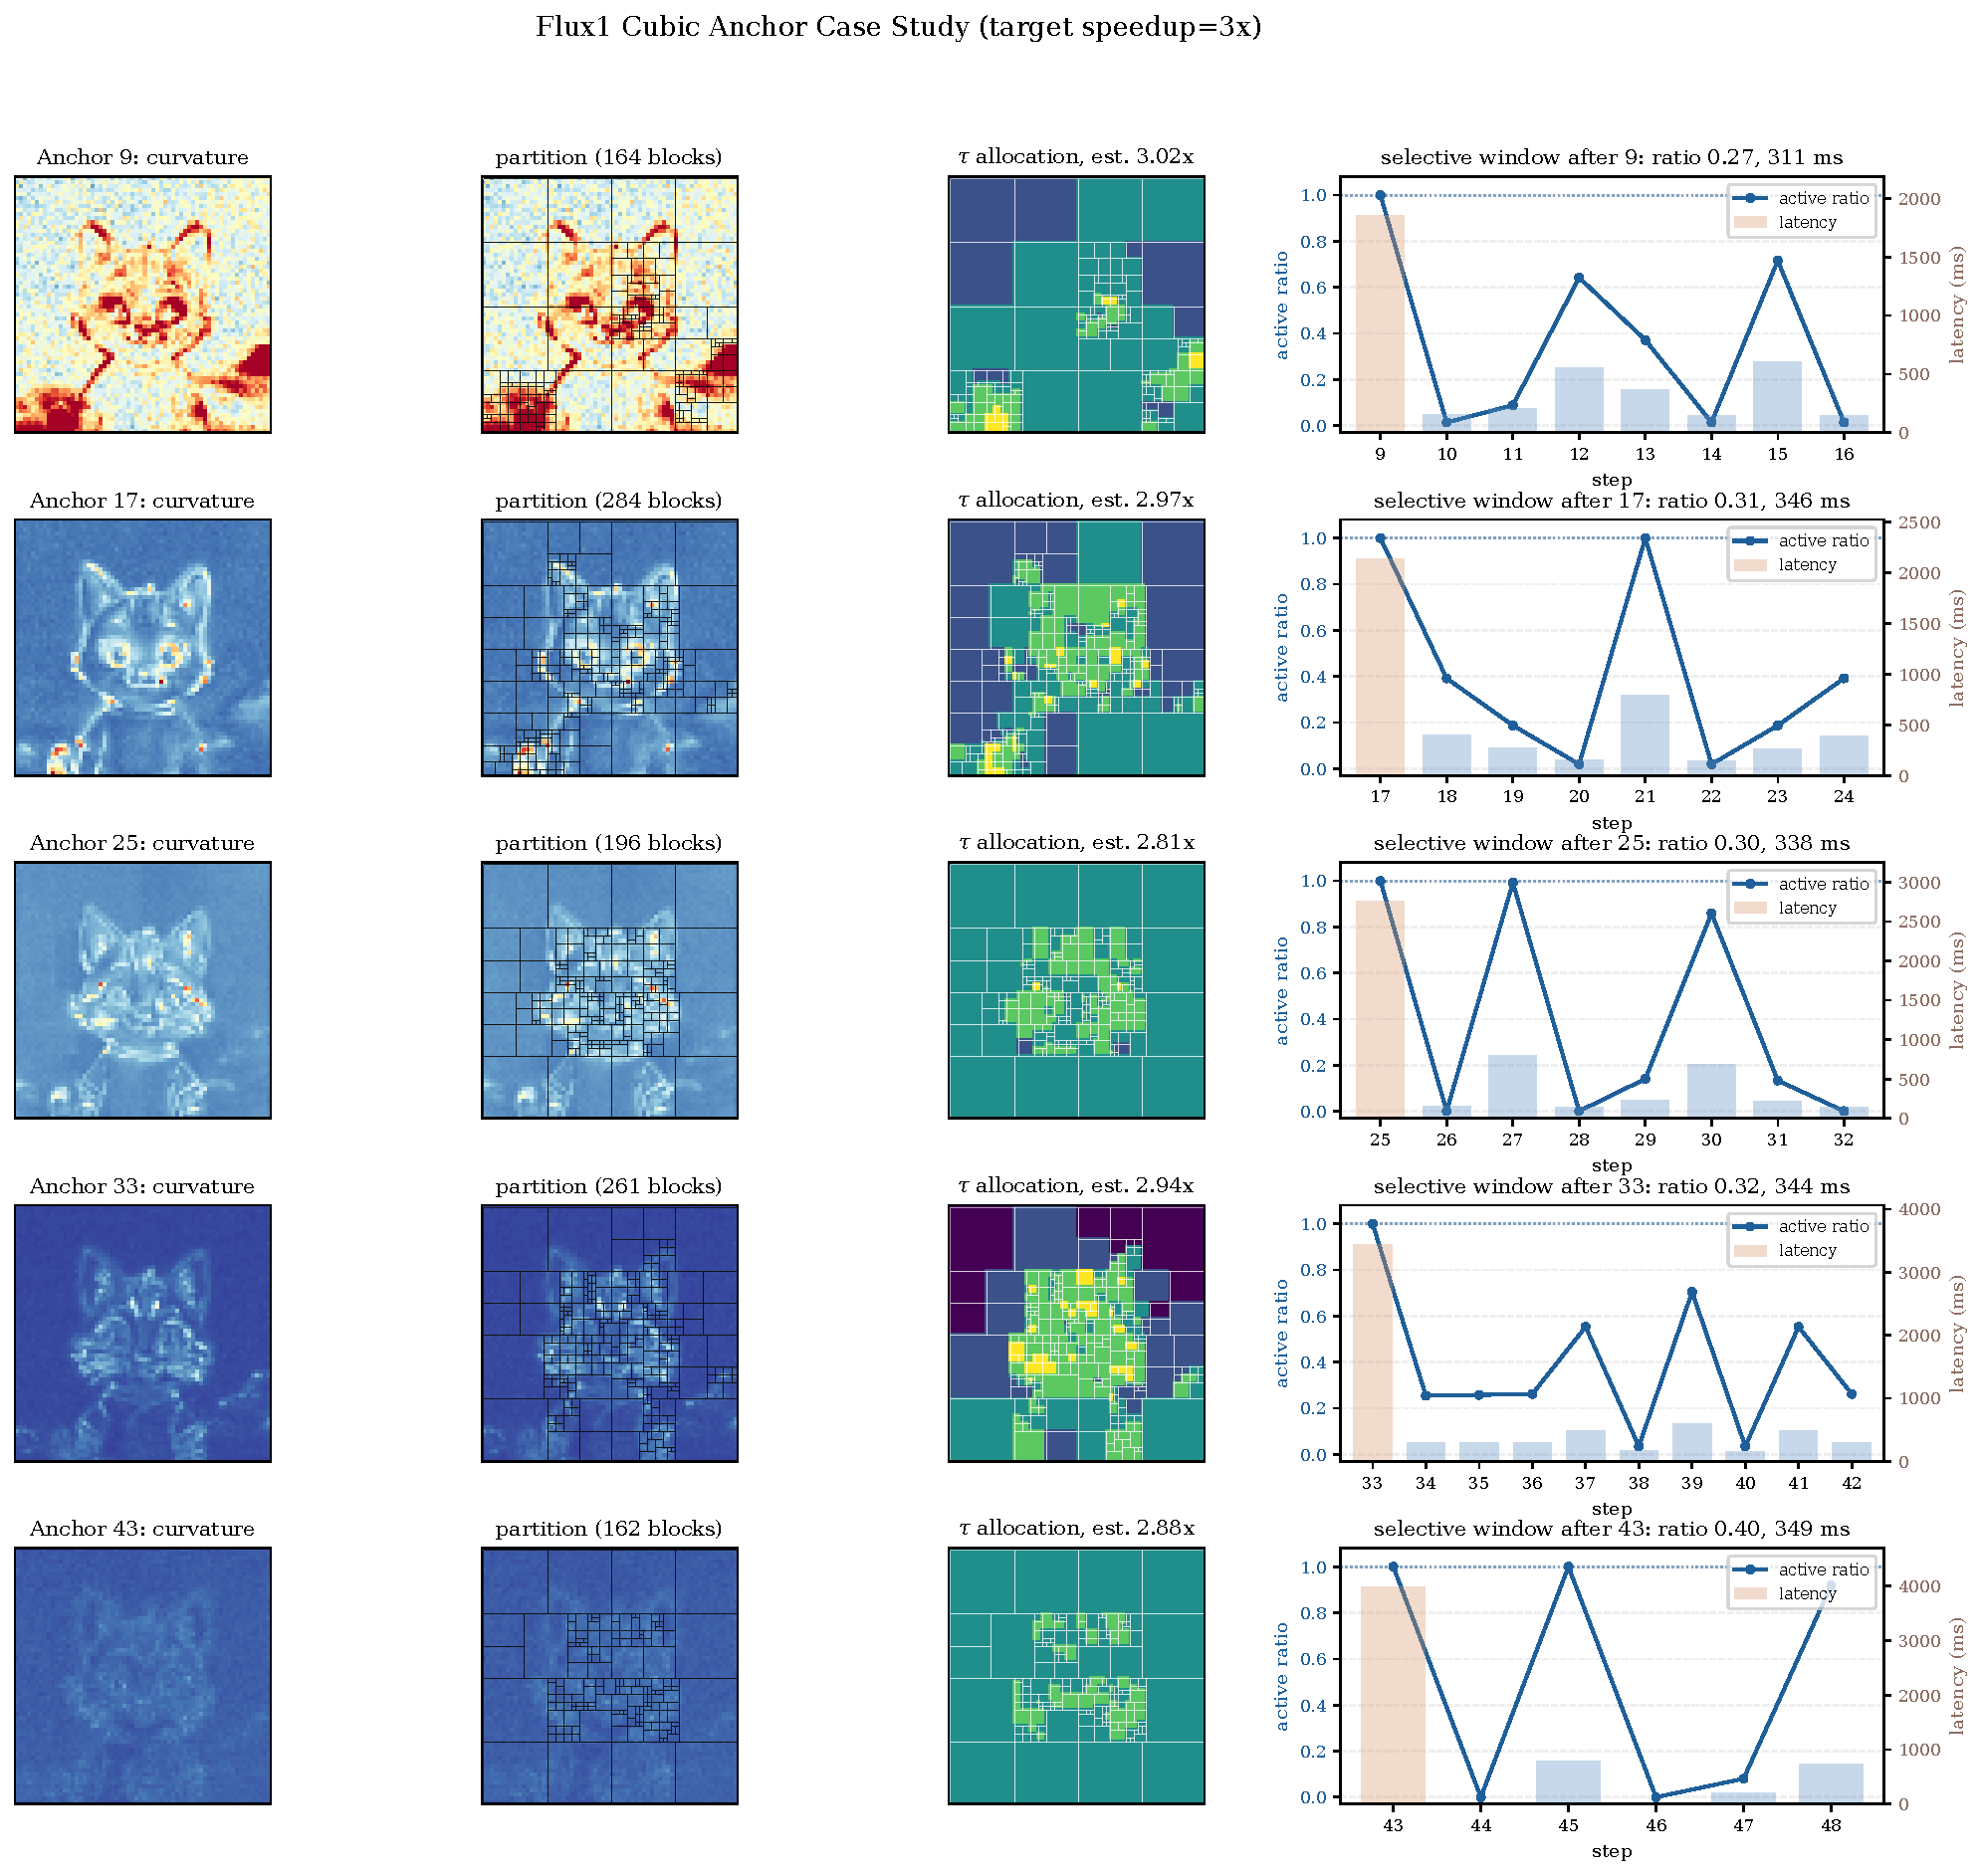
\includegraphics[width=\linewidth]{figure/casestudy.pdf}
    \caption{\cubic case study on Flux.1 with target speedup $3\times$.}
    \label{fig:case_study}
\end{figure}


\newpage
\section{Detailed Results of \cubic Evaluation}
\label{app:detail_result}
We report the detailed parameter settings and performance of \cubic in Table~\ref{tab:detail}. For completeness, Table~\ref{tab:detail_baseline} provides the corresponding configurations and results of other baseline methods.

\begin{table*}[h]
\centering
\caption{Parameters setting and performance of \cubic }
\label{tab:detail}´
\resizebox{0.7\textwidth}{!}{
\begin{tabular}{l c c c c c c}
\toprule
\small
\textbf{Model}
& $\boldsymbol{\rho}$
& $\mathrm{Speedup}\uparrow$
& $\mathrm{PSNR}\uparrow$
& $\mathrm{SSIM}\uparrow$
& $\mathrm{LPIPS}\downarrow$
& $\mathrm{FID/FVD}\downarrow$ \\
\midrule

% ===== Flux-1 =====
\multirow{5}{*}{Flux-1}
& 2  & 1.38$\times$ & 32.03 & 0.9445 & 0.0409 & 12.51 \\
& 4  & 1.89$\times$ & 27.78 & 0.8998 & 0.0946 & 27.81 \\
& 6  & 2.22$\times$ & 26.04 & 0.8691 & 0.1299 & 37.14 \\
& 8  & 2.40$\times$ & 25.14 & 0.8457 & 0.1730 & 47.32 \\
& 10 & 2.51$\times$ & 24.45 & 0.8282 & 0.1964 & 52.82 \\
\midrule

% ===== FireRed =====
\multirow{5}{*}{FireRed}
& 2  & 1.76$\times$ & 33.85 & 0.9711 & 0.0268 & 10.91 \\
& 4  & 2.14$\times$ & 30.67 & 0.9538 & 0.0468 & 18.55 \\
& 6  & 2.23$\times$ & 28.74 & 0.9310 & 0.0769 & 27.15 \\
& 8  & 2.33$\times$ & 27.81 & 0.9201 & 0.0907 & 32.18 \\
& 10 & 2.50$\times$ & 27.06 & 0.9080 & 0.1059 & 38.35 \\
\midrule

% ===== Wan-1.3B =====
\multirow{5}{*}{Wan-1.3B}
& 2  & 1.63$\times$ & 32.76 & 0.9481 & 0.0317 & 7.912 \\
& 4  & 2.30$\times$ & 27.99 & 0.8990 & 0.0728 & 21.14 \\
& 6  & 2.72$\times$ & 26.39 & 0.8740 & 0.0986 & 31.76 \\
& 8  & 3.04$\times$ & 25.50 & 0.8501 & 0.1236 & 45.08 \\
& 10 & 3.23$\times$ & 24.65 & 0.8284 & 0.1437 & 62.48 \\

\bottomrule
\end{tabular}
}
\end{table*}

\begin{table*}[h]
\centering
\caption{Parameters setting and performance of baselines. }
\label{tab:detail_baseline}
\resizebox{0.7\textwidth}{!}{
\begin{tabular}{l l c c c c c}
\toprule
\textbf{Model} & \textbf{Method}
& $\mathrm{Speedup}\uparrow$
& $\mathrm{PSNR}\uparrow$
& $\mathrm{SSIM}\uparrow$
& $\mathrm{LPIPS}\downarrow$
& $\mathrm{FID/FVD}\downarrow$ \\
\midrule

\multirow{12}{*}{\textbf{Flux-1}}
& ToCa(4)         & 1.69$\times$ & 20.34 & 0.7647 & 0.2414 & 61.97 \\
& ToCa(5)         & 1.81$\times$ & 19.68 & 0.7493 & 0.2726 & 70.76\\
& ToCa(6)         & 1.93$\times$ & 18.88 & 0.7094 & 0.3164 & 78.10 \\
& TeaCache(0.25)  & 1.86$\times$ & 22.88 & 0.8514 & 0.1490 & 45.87 \\
& TeaCache(0.4)   & 2.52$\times$ & 19.66 & 0.7720 & 0.2481 & 66.04 \\
& TeaCache(0.6)   & 3.31$\times$ & 17.66 & 0.7279 & 0.3155 & 89.86 \\
& TaylorSeer(N2)  & 1.70$\times$ & 26.29 & 0.8920 & 0.0994 & 26.80 \\
& TaylorSeer(N3)  & 2.25$\times$ & 21.42 & 0.8180 & 0.1796 & 47.53 \\
& TaylorSeer(N4)  & 2.66$\times$ & 19.27 & 0.7606 & 0.2497 & 63.59 \\
& PAB(4)          & 1.62$\times$ & 22.88 & 0.8373 & 0.1613 & 47.83 \\
& PAB(8)          & 1.81$\times$ & 20.37 & 0.7702 & 0.2574 & 77.37 \\
& PAB(12)         & 1.90$\times$ & 19.47 & 0.7344 & 0.3293 & 106.65 \\
\midrule

\multirow{13}{*}{\textbf{FireRed}}
& ToCa(3)     & 1.50$\times$ & 24.17 & 0.8736 & 0.1103 & 49.84 \\
& ToCa(4)     & 1.76$\times$ & 22.57 & 0.8367 & 0.1471 & 62.58 \\
& ToCa(5)     & 1.95$\times$ & 21.09 & 0.7884 & 0.1779 & 67.25 \\
& TeaCache(0.1)   & 1.51$\times$ & 27.49 & 0.9363 & 0.0562 & 25.55 \\
& TeaCache(0.15)  & 2.04$\times$ & 25.65 & 0.9183 & 0.0758 & 31.00 \\
& TeaCache(0.2)   & 2.31$\times$ & 23.80 & 0.8955 & 0.0995 & 41.03 \\
& TaylorSeer(N2)  & 1.86$\times$ & 25.12 & 0.9102 & 0.0837 & 33.70 \\
& TaylorSeer(N3)  & 2.64$\times$ & 21.17 & 0.8356 & 0.1498 & 50.38 \\
& TaylorSeer(N4)  & 3.35$\times$ & 18.96 & 0.7774 & 0.1987 & 64.84 \\
& PAB(6)          & 1.61$\times$ & 25.82 & 0.9112 & 0.0731 & 33.92 \\
& PAB(8)          & 1.65$\times$ & 24.39 & 0.8888 & 0.0929 & 39.41 \\
& PAB(12)         & 1.68$\times$ & 22.45 & 0.8530 & 0.1312 & 54.07 \\
& PAB(16)         & 1.72$\times$ & 20.87 & 0.9198 & 0.1799 & 67.82 \\
\midrule

\multirow{12}{*}{\textbf{Wan1.3B}}
& ToCa(242)        & 1.69$\times$ & 19.60 & 0.7486 & 0.2273 & 78.95 \\
& ToCa(333)        & 2.21$\times$ & 20.66 & 0.7684 & 0.1949 & 66.02 \\
& ToCa(363)        & 2.31$\times$ & 19.19 & 0.7383 & 0.2405 & 84.04 \\
& TeaCache(0.05)   & 1.65$\times$ & 30.27 & 0.9270 & 0.0454 & 11.72 \\
& TeaCache(0.07)   & 1.75$\times$ & 26.38 & 0.8684 & 0.0933 & 24.85 \\
& TeaCache(0.08)   & 2.15$\times$ & 24.51 & 0.8405 & 0.1206 & 35.26 \\
& TaylorSeer(N2)   & 1.91$\times$ & 18.29 & 0.7225 & 0.2504 & 94.59 \\
& TaylorSeer(N3)   & 2.59$\times$ & 15.80 & 0.6410 & 0.3521 & 137.06 \\
& TaylorSeer(N4)   & 3.19$\times$ & 14.04 & 0.5837 & 0.4406 & 181.41 \\
& PAB(2,5)         & 1.67$\times$ & 24.06 & 0.8370 & 0.1212 & 36.82 \\
& PAB(4,5)         & 2.17$\times$ & 22.83 & 0.8127 & 0.1530 & 52.37 \\
& PAB(6,6)         & 2.50$\times$ & 22.36 & 0.8000 & 0.1670 & 57.78 \\
\bottomrule
\end{tabular}
}
\end{table*}

\newpage

\section{Visualization of \cubic}
\label{app_vis}
We provide visualization comparison between original video generation and \cubic on Flux-1, FireRed and Wan 2.1. We evaluate \cubic on Text-to-Image generation, Image Editing, and Text-to-Video generation using the default resolution of each model. Results demonstrates \cubic can preserve high pixel-level fidelity, achieving similar generation quality compared with the original generation.
\begin{figure*}[!h]
    \centering
    \includegraphics[width=\textwidth]{figure/flux_ori_cubic_comparison.pdf}
    \caption{Flux visualization comparison between original images (top) and \cubic results (bottom)}
    \label{fig:flux_visual}
\end{figure*}

\begin{figure*}[!h]
    \centering
    \includegraphics[width=\textwidth]{figure/firered_ori_cubic_comparison.pdf}
    \caption{FireRed visualization comparison between original images (top) and \cubic results (bottom)}
    \label{fig:firered_visual}
\end{figure*}

\begin{figure*}[!h]
    \centering
    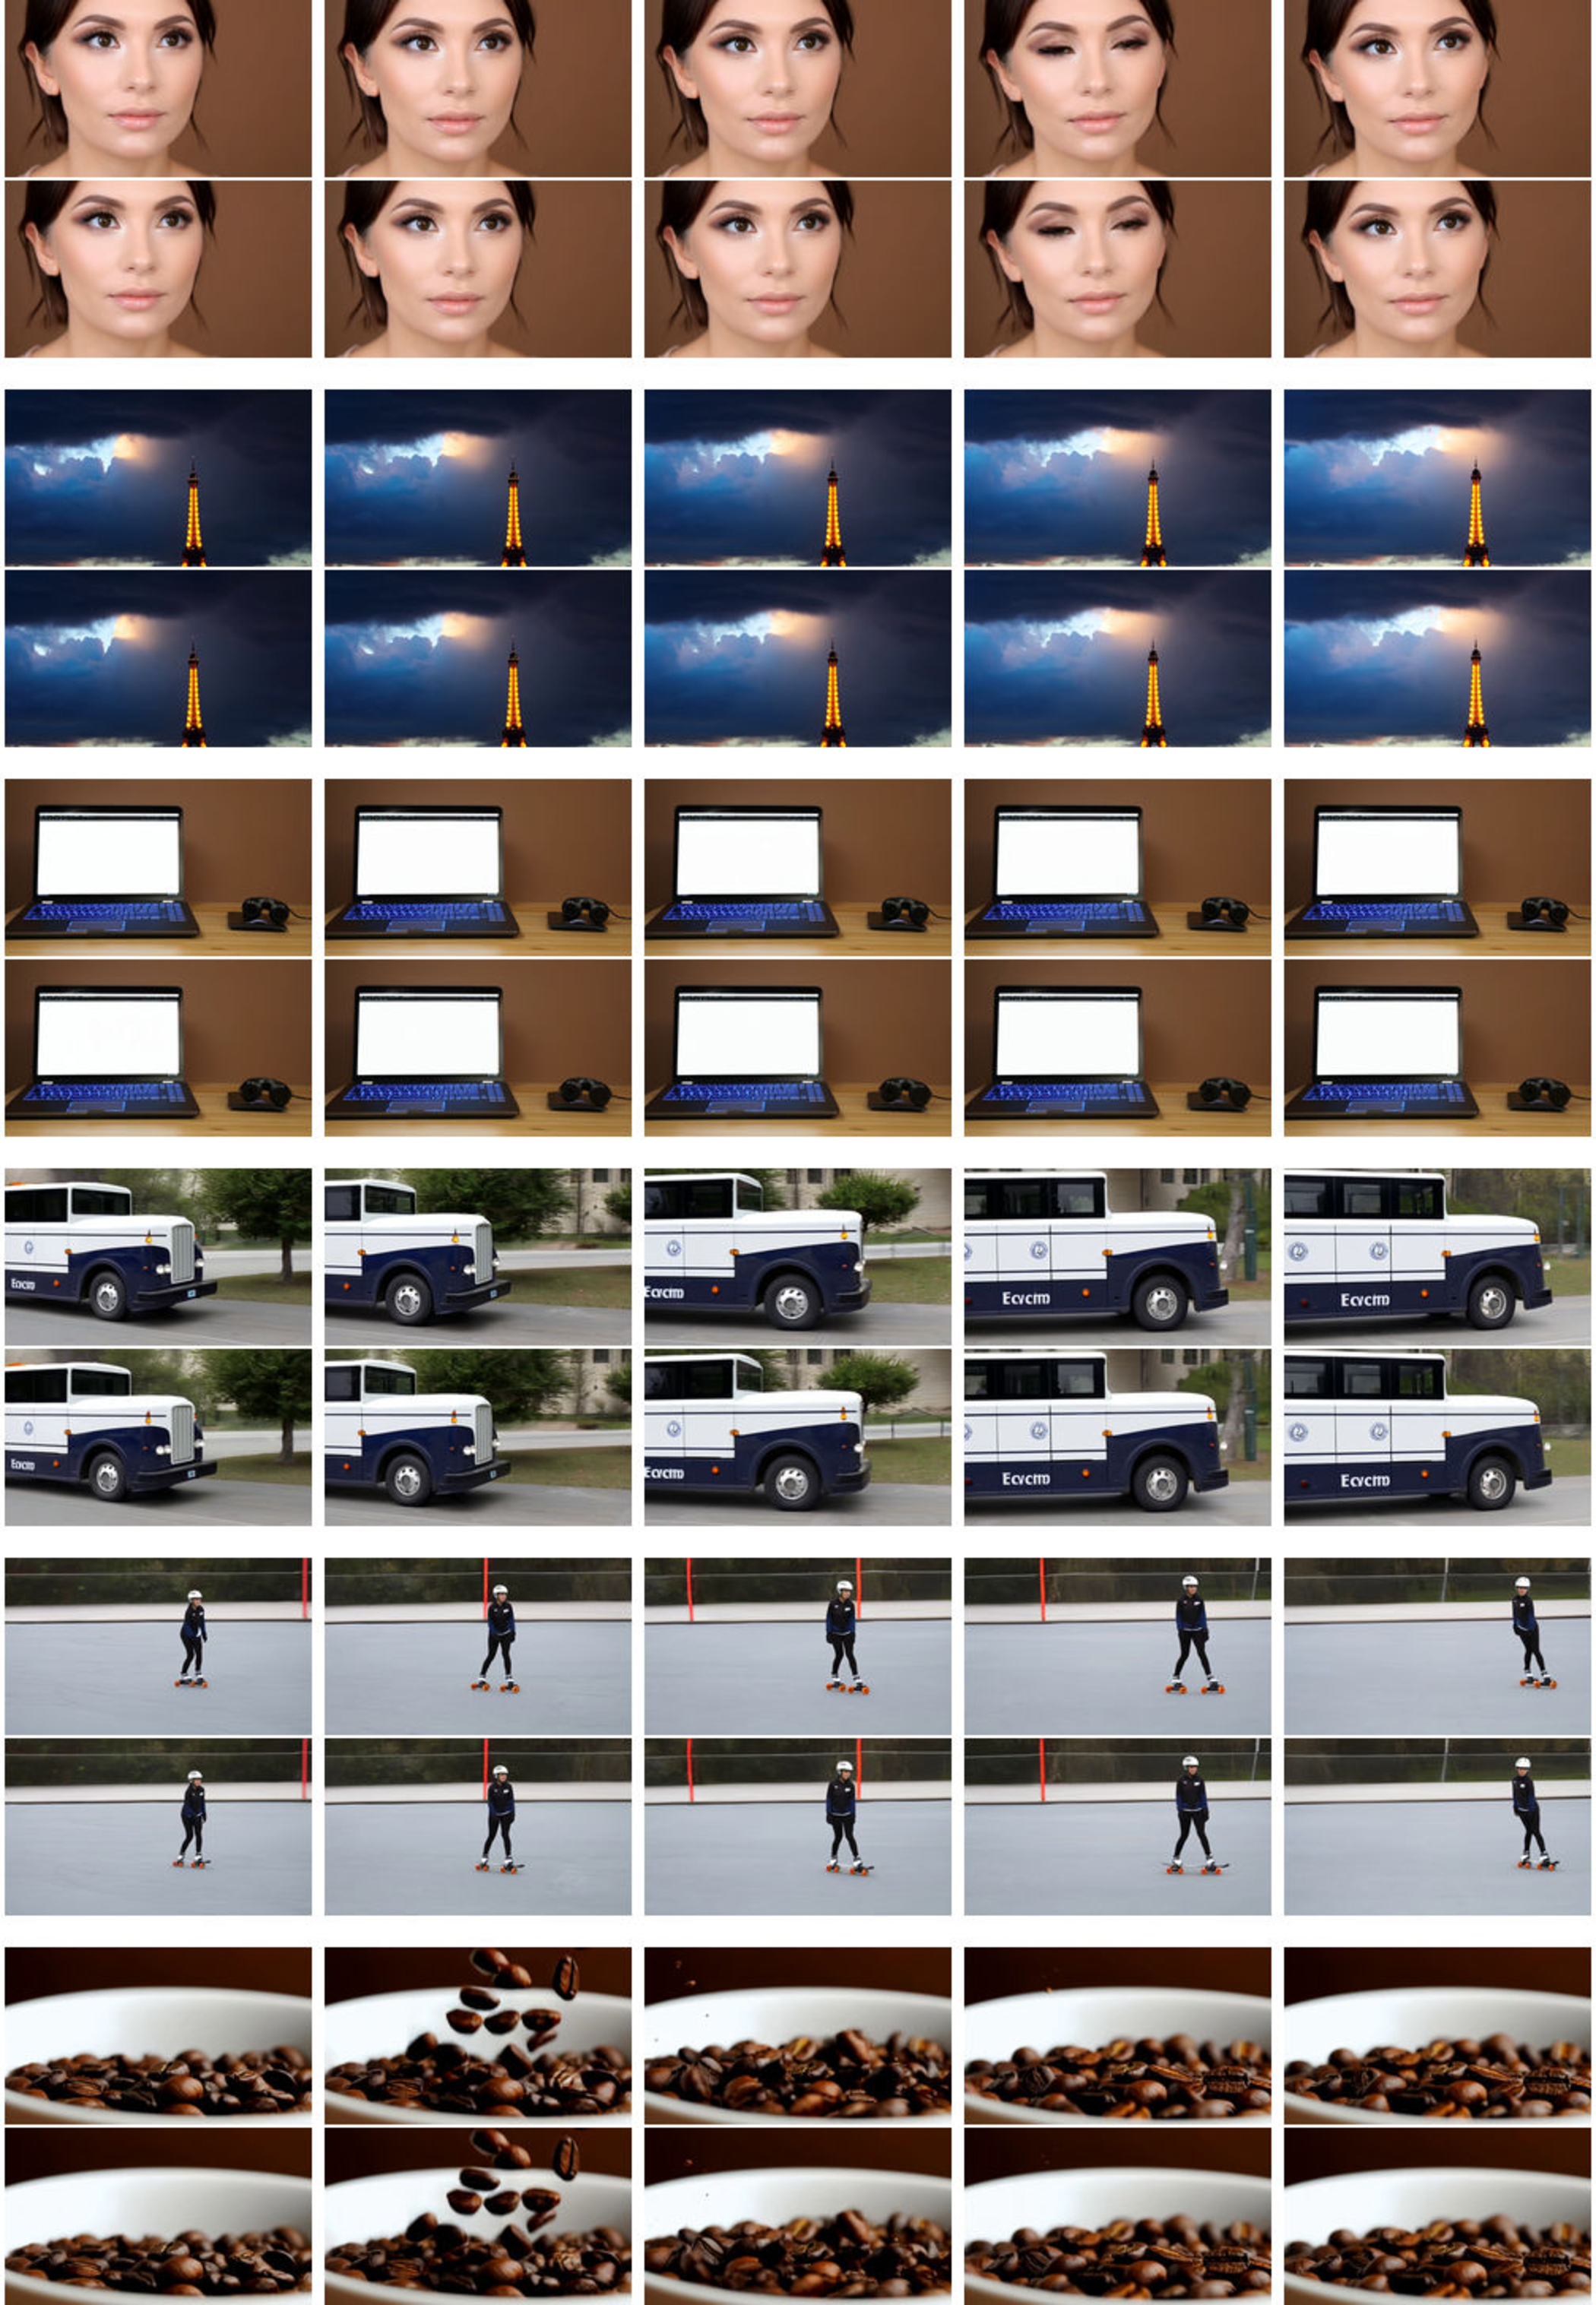
\includegraphics[width=\textwidth]{figure/wan_ori_cubic_video_comparison.pdf}
    \caption{Wan 1.3B visualization comparison between original vedios (top) and \cubic results (bottom)}
    \label{fig:wan_visual}
\end{figure*}
